\chapter{От принципа эквивалентности к тензорам}

Общую теорию относительности обычно сокращают как GR, хотя специальную теорию относительности редко называют SR. Это сокращение менее важно, чем решение начать с самого начала. Самый прямой путь — тот, которым пошел Эйнштейн: начать с физического наблюдения, достаточно простого, чтобы его можно было ощутить в лифте, довести его до точки, где его следствия становятся неизбежными, и лишь затем вводить геометрию.

Первое наблюдение — это принцип эквивалентности. Гравитация и ускорение локально неразличимы. Слово локально в конце концов возьмет на себя почти всю нагрузку этого утверждения. Однако, прежде чем вводить это уточнение, стоит увидеть, что уже может дать формулировка без него.

\section{Лифт как преобразование координат}

В учебниках лифт Эйнштейна часто заменяют ракетой. Здесь лифт предпочтительнее, потому что его ускорение нам привычно. Пусть \(z\) измеряет высоту в системе отсчета, связанной с землей, а \(z'\) измеряет высоту от пола лифта. Если пол имеет высоту \(L(t)\), то одно и то же событие имеет координаты \begin{equation}
 z'=z-L(t),\qquad t'=t,\qquad x'=x.
\label{eq:elevator-map}
\end{equation} Горизонтальная координата не изменяется, потому что лифт не смещается в сторону. Выбор \(t'=t\) намеренно пока оставляет специальную теорию относительности в стороне.

\begin{classroomqa}\audiencequestion{Как курс по общей теории относительности может начинаться с игнорирования специальной теории относительности?}\lecturerresponse{Существует режим, в котором гравитация существенна, тогда как все скорости остаются малы по сравнению с \(c\). Поэтому связь гравитации--ускорения можно выделить в ньютоновской механике, а затем объединить с геометрией Минковского. Это выбор порядка изложения, а не утверждение, что окончательная теория нерелятивистская. \lecturetimestamp{00:05:33}}\end{classroomqa}

В двух инерциальных системах отсчета лифт движется равномерно: \begin{equation}
 L(t)=vt,\qquad z'=z-vt.
\label{eq:galilean-elevator}
\end{equation} Начала координат выбраны совпадающими при \(t=0\). На доске рисунок лифта оставлен рядом со всеми тремя соотношениями между координатами, чтобы символы никогда не теряли своего физического смысла.

\begin{figure}[H]\centering
\includegraphics[width=\linewidth]{lecture_01_figure_01.png}\caption{Координаты лифта после специализации к случаю равномерного движения \(L(t)=vt\).}\par\smallskip
\textit{Кадр лекции: 00:09:10.}\end{figure}

Рассмотрим только вертикальную компоненту закона Ньютона: \begin{equation}
 F=m\ddot z.
\label{eq:newton-unprimed}
\end{equation} Сила может возникать из-за веревки, электрического поля или любого другого обычного взаимодействия. Двукратное дифференцирование \eqref{eq:galilean-elevator} дает \(\ddot z'=\ddot z\), а следовательно, \begin{equation}
 F=m\ddot z'.
\label{eq:newton-primed-inertial}
\end{equation} Вид закона не изменяется. Это элементарное вычисление выявляет операционное содержание эквивалентности инерциальных систем отсчета: линейное преобразование координат переводит равномерное движение в равномерное.

\begin{figure}[H]\centering
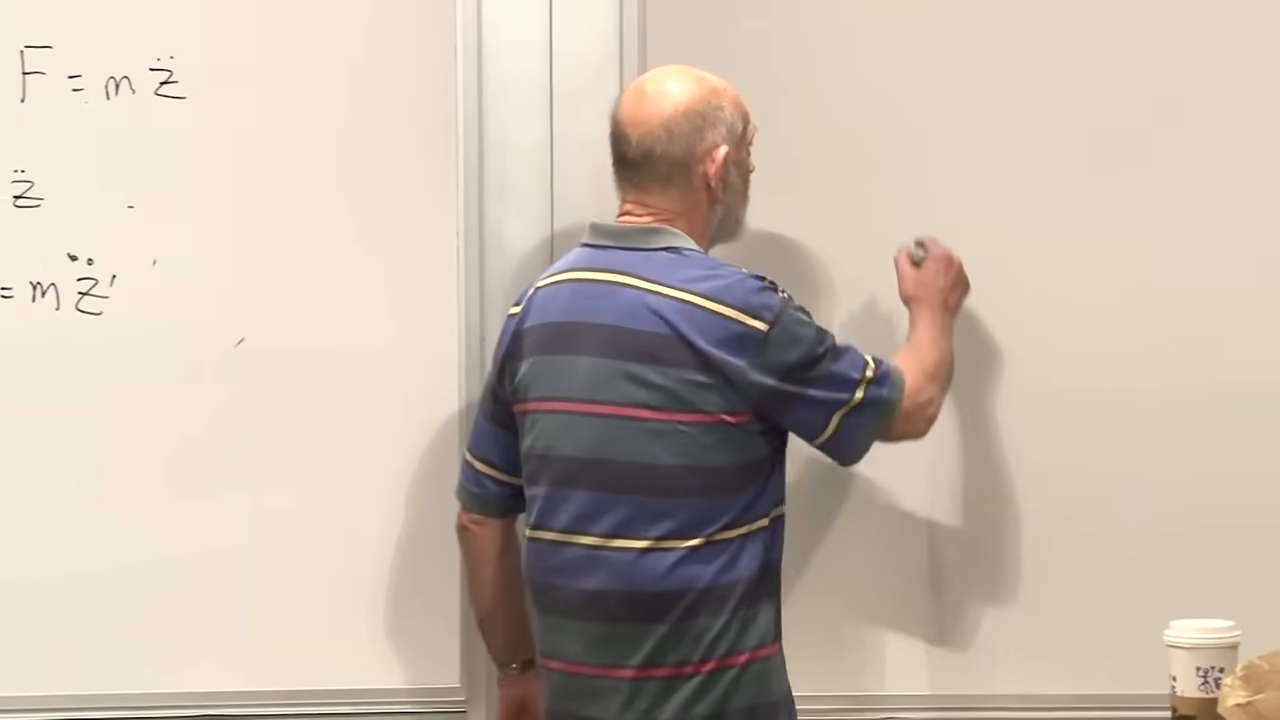
\includegraphics[width=\linewidth]{lecture_01_figure_02.png}\caption{Уравнение Ньютона в двух равномерно движущихся системах координат.}\par\smallskip
\textit{Кадр лекции: 00:11:50.}\end{figure}

Теперь сообщим лифту направленное вверх постоянное ускорение \(g\): \begin{equation}
 L(t)=\frac12gt^2,\qquad
 \dot L=gt,\qquad
 \ddot L=g.
\end{equation} Преобразование координат принимает вид \begin{equation}
 z'=z-\frac12gt^2,
\qquad
 \ddot z'=\ddot z-g.
\label{eq:accelerated-map}
\end{equation} Подстановка в закон Ньютона дает \begin{equation}
 F=m(\ddot z'+g),
\qquad
 m\ddot z'=F-mg.
\label{eq:fictitious-gravity}
\end{equation} В выводе есть полезная проверка знака по ходу дела: \(+mg\) сначала появляется в части уравнения с ускорением и превращается в \(-mg\) только после переноса в часть с силой. Окончательное направление — вниз в системе отсчета, пол которой ускоряется вверх.

\begin{figure}[H]\centering
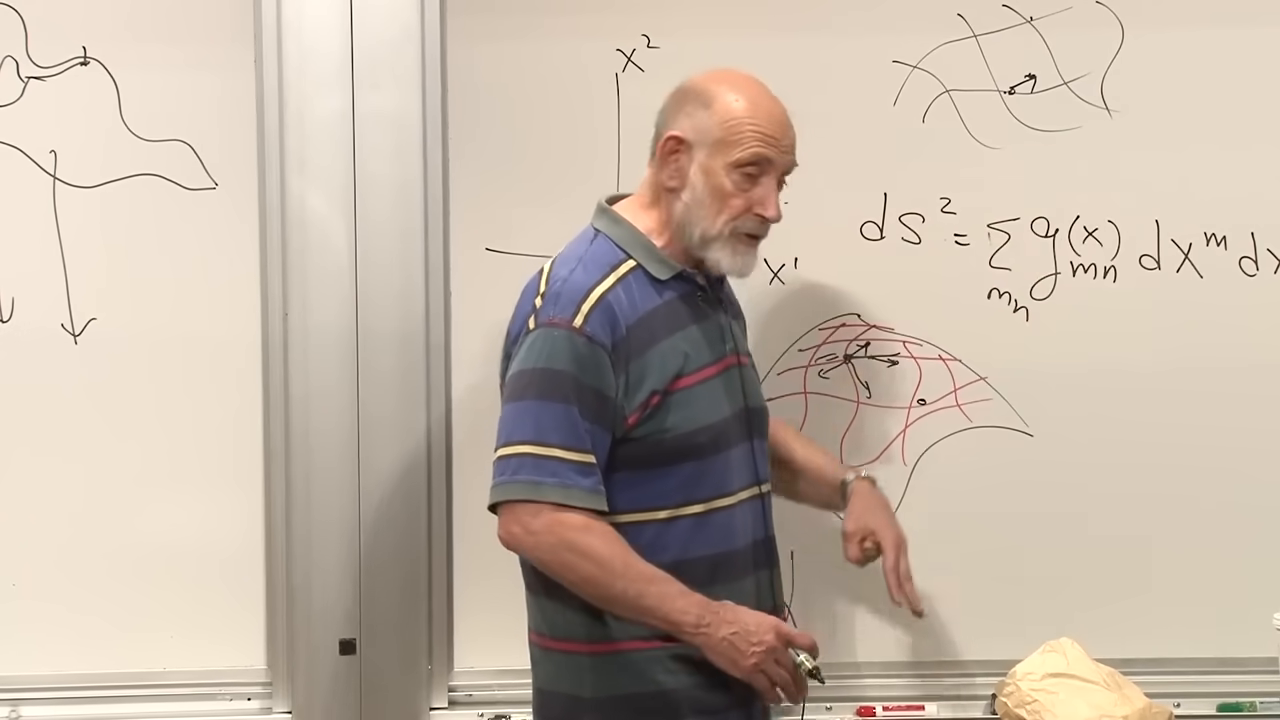
\includegraphics[width=\linewidth]{lecture_01_figure_03.png}\caption{Ускоренное преобразование и возникающая при этом фиктивная сила \(-mg\).}\par\smallskip
\textit{Кадр лекции: 00:15:35.}\end{figure}

Новый член выглядит гравитационным по вполне определенной причине: он пропорционален массе. Поскольку инерционный отклик также пропорционален массе, масса сокращается в уравнении движения. Свободно падающее тело движется по одной и той же траектории независимо от своей массы. Орбита Земли, например, определяется ее положением и скоростью в поле Солнца, а не собственной массой Земли в приближении пробного тела.

До Эйнштейна это сходство можно было счесть любопытной случайностью. Эйнштейн же возвел его в принцип: никакой локальный механический эксперимент не может отличить однородное гравитационное поле от подходящим образом ускоренной системы отсчета.

\section{Прямые линии, криволинейные координаты и свет}

Отложим \(t\) по вертикали, а \(z\) по горизонтали. При \(z'=z-vt\) линии постоянного \(z'\) являются параллельными прямыми. Прямые мировые линии остаются прямыми, потому что преобразование координат линейно.

\begin{figure}[H]\centering
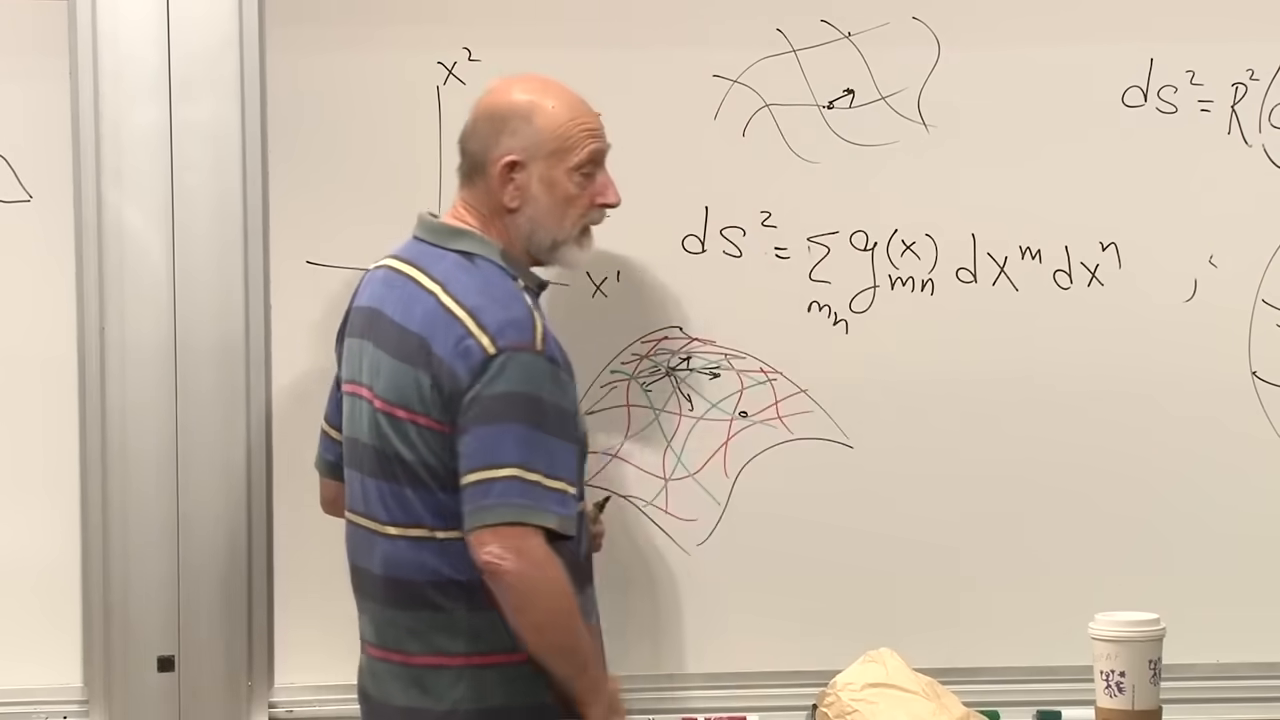
\includegraphics[width=\linewidth]{lecture_01_figure_04.png}\caption{Линейная пространственно-временная сетка для равномерно движущихся систем координат.}\par\smallskip
\textit{Кадр лекции: 00:19:45.}\end{figure}

Для ускоренного отображения линия постоянного \(z'\) удовлетворяет соотношению \begin{equation}
 z=z'+\frac12gt^2.
\end{equation} Это парабола, лежащая на боку. Продлевая движение назад во времени, получаем лифт, который спускается, замедляясь, разворачивается, а затем ускоряется вверх. Каждая соседняя линия постоянного \(z'\) — та же самая парабола, сдвинутая по горизонтали.

\begin{figure}[H]\centering
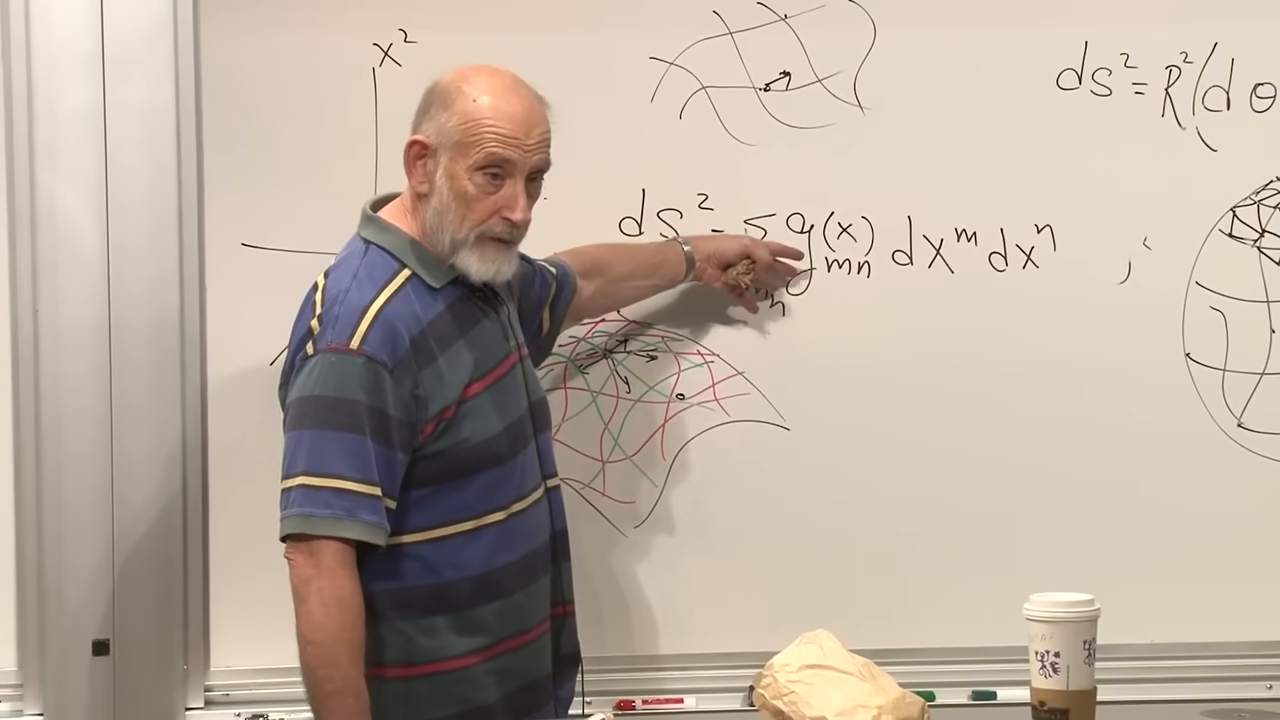
\includegraphics[width=\linewidth]{lecture_01_figure_05.png}\caption{Кривые постоянного \(z'\) для равномерно ускоренной системы координат.}\par\smallskip
\textit{Кадр лекции: 00:22:25.}\end{figure}

Это первая геометрическая подсказка. В специальной теории относительности используются линейные преобразования Лоренца, которые переводят прямые линии пространства-времени в прямые линии пространства-времени. Чтобы представлять ускорение и тем самым имитировать гравитацию, нужны криволинейные преобразования пространственно-временных координат.

Эйнштейн использовал этот, казалось бы, скромный пункт, чтобы ответить на вопрос, который был совсем не скромным: влияет ли гравитация на свет? В момент \(t=0\) пусть система лифта и система, связанная с землей, мгновенно покоятся друг относительно друга, и пустим поперек лифта горизонтальный луч света. В неускоренной системе отсчета \begin{equation}
 x=ct,\qquad z=0.
\end{equation} Используя \(z=z'+\tfrac12gt^2\), получаем, что тот же луч в координатах лифта удовлетворяет \begin{equation}
 z'=-\frac12gt^2
    =-\frac{g}{2c^2}x^2.
\label{eq:accelerated-light}
\end{equation} Световой луч прямой в инерциальной системе и искривлен в ускоренной. Если ускорение и гравитация локально эквивалентны, гравитационное поле должно искривлять свет. Этот аргумент устанавливает эффект еще до того, как записано какое-либо уравнение поля для гравитации.

\begin{figure}[H]\centering
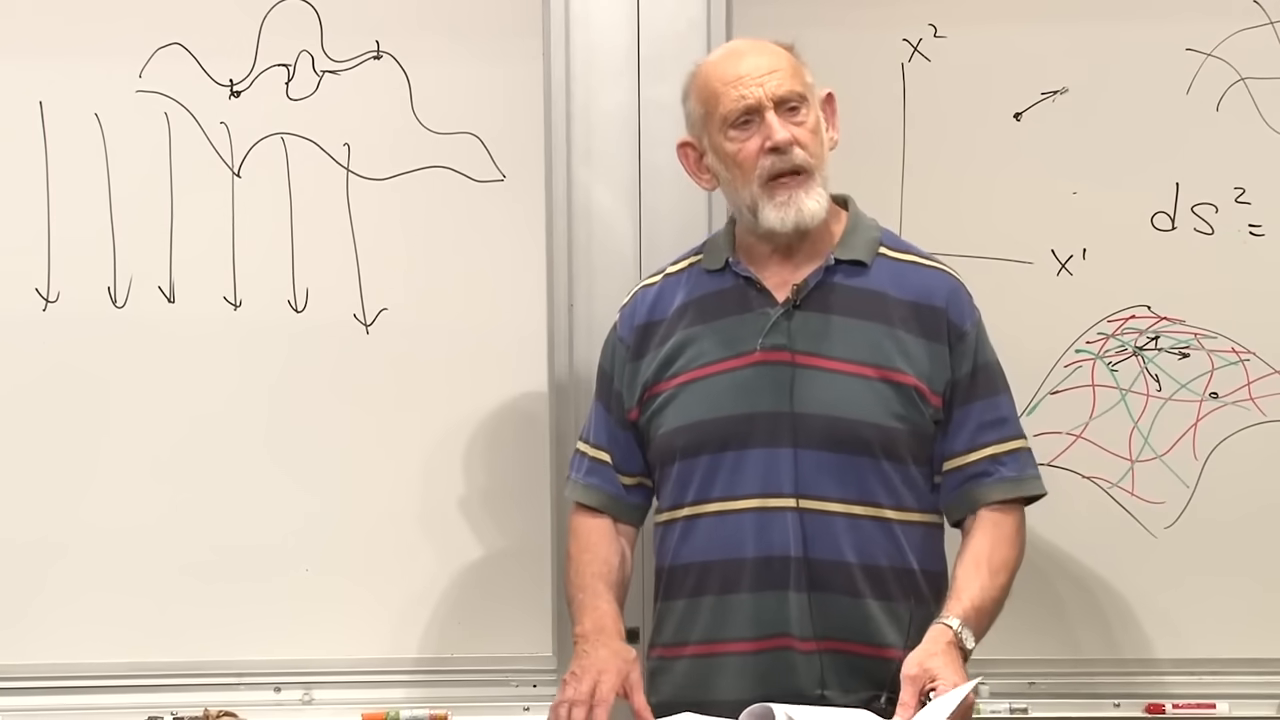
\includegraphics[width=\linewidth]{lecture_01_figure_06.png}\caption{Горизонтальный световой луч и его искривленная траектория в ускоренной системе отсчета.}\par\smallskip
\textit{Кадр лекции: 00:28:10.}\end{figure}

\section{Что нельзя устранить преобразованием}

Ускоренная система отсчета может создать кажущееся однородное гравитационное поле. Из этого не следует, что всякое гравитационное поле есть артефакт выбора координат. Поле звезды направлено радиально внутрь. Небольшая свободно падающая лаборатория вблизи одной точки может устранить локальное ускорение, но то же преобразование не может устранить поле со всех сторон звезды.

\begin{figure}[H]\centering
\includegraphics[width=\linewidth]{lecture_01_figure_07.png}\caption{Радиальное поле и протяженное падающее тело, используемые для выявления приливного ускорения.}\par\smallskip
\textit{Кадр лекции: 00:32:50.}\end{figure}

Препятствием служит приливная сила. Представьте человека ростом в две тысячи миль, падающего ногами вниз. Его ноги ближе к источнику и ускоряются сильнее, чем голова, поэтому он растягивается. Поверните его боком, и направления внутрь на противоположных сторонах будут иметь составляющие, направленные друг к другу, так что он сжимается. На языке ньютоновской механики соседние точки, разделенные \(\xi^j\), приобретают относительное ускорение \begin{equation}
 \delta a^i \simeq \partial_j g^i\,\xi^j.
\label{eq:newtonian-tide}
\end{equation} Координатное ускорение можно устранить. Относительное ускорение в пределах протяженного свободно падающего тела — нельзя.

\begin{classroomqa}\audiencequestion{Могли бы разные ракетные двигатели у головы и у ног имитировать растяжение и тем самым имитировать приливное поле?}\lecturerresponse{Такие двигатели, конечно, могут создавать напряжения в теле, но это реальная негравитационная сила, по-разному действующая на его части. Одно лишь изменение координат не может создать инвариантное относительное ускорение между соседними свободно падающими частицами. Речь в этом критерии идет о свободном падении без приложенных сил, а не о теле, приводимом в движение отдельными ракетами. \lecturetimestamp{00:36:51}}\end{classroomqa}

Криволинейные координаты, тем не менее, могут придавать фиктивным полям весьма сложный вид. Система отсчета может ускоряться по вертикали, одновременно колеблясь по горизонтали и создавая зависящее от времени кажущееся поле с обеими компонентами. Даже обычные полярные координаты дают поучительный пример. Свободная частица, движущаяся по прямой линии в декартовых координатах, сначала имеет убывающий \(r(t)\), достигает минимального радиуса, а затем \(r(t)\) возрастает. Тот, кому известны только \(r(t)\) и \(\theta(t)\), мог бы заключить, что действует направленная наружу отталкивающая сила. Во вращающихся вариантах этих координат появляются центробежный и кориолисов члены. Они пропорциональны массе и поэтому выглядят гравитационными, но не оставляют на свободно падающем теле никакой инвариантной приливной деформации.

\begin{classroomqa}
\audiencequestion{Что происходит, если движение описывать в угловых или полярных координатах?}
\lecturerresponse{Нелинейное координатное описание заставляет прямолинейную свободную траекторию выглядеть так, как будто она отталкивается от \(r=0\). Эта эффективная центробежная сила является координатной силой. Возвращение к инерциальной декартовой системе отсчёта устраняет её и показывает, что никаких приливных искажений нет.
\lecturetimestamp{00:37:56}}
\end{classroomqa}

\begin{figure}[H]
\centering
\includegraphics[width=\linewidth]{lecture_01_figure_08.png}
\caption{Описание прямолинейной траектории в полярных координатах; на доске отмечены \(r(t)\) и \(\theta(t)\).}
\par\smallskip
\textit{Кадр лекции: 00:40:20.}
\end{figure}

\begin{classroomqa}
\audiencequestion{Могут ли несколько гравитирующих тел взаимно компенсировать друг друга и не оставить приливной силы?}
\lecturerresponse{Силы могут компенсироваться в выбранной точке, но компенсация значения поля, вообще говоря, не компенсирует его пространственные производные. Вблизи любого отдельного источника соседние траектории всё равно получают разные ускорения. Истинное отсутствие кривизны требует, чтобы приливной диагностический критерий обращался в нуль во всей области, а не только чтобы результирующая сила в одной точке была равна нулю. \lecturetimestamp{00:42:16}}
\end{classroomqa}

\begin{classroomqa}
\audiencequestion{Как операционально измеряют приливную силу?}
\lecturerresponse{Отпустите протяжённый объект, например кристалл, в свободное падение и посмотрите, появляются ли напряжения и деформации, которые растягивают его в одном направлении и сжимают в другом. Эти деформации измеримы и не исчезают при переименовании координат. \lecturetimestamp{00:44:38}}
\end{classroomqa}

\begin{classroomqa}
\audiencequestion{Почувствовал бы человек размером в две тысячи миль на карусели радиальный приливной эффект?}
\lecturerresponse{Человек, привязанный к карусели, испытывает силы со стороны опоры, и у него вполне может разболеться голова. Однако пробное тело должно находиться в свободном падении. В вращающихся координатах его траектория выглядит сложной, но в инерциальной системе отсчёта остаётся прямолинейной траекторией без напряжений, так что инвариантная приливная сила равна нулю.
\lecturetimestamp{00:45:07}}
\end{classroomqa}

\begin{classroomqa}
\audiencequestion{Можно ли наклонить падающее тело так, чтобы растяжение и сжатие компенсировались?}
\lecturerresponse{Никакая отдельная ориентация не устраняет деформацию полностью. Радиальное поле растягивает вдоль одного главного направления и сжимает вдоль поперечных направлений. Тело конечных размеров во всех направлениях испытывает всю эту картину целиком. \lecturetimestamp{00:47:10}}
\end{classroomqa}

\begin{figure}[H]
\centering
\includegraphics[width=\linewidth]{lecture_01_figure_09.png}
\caption{Для протяжённого свободно падающего тела одновременно показаны радиальное растяжение и поперечное сжатие.}
\par\smallskip
\textit{Кадр лекции: 00:47:55.}
\end{figure}

\begin{classroomqa}
\audiencequestion{Означают ли приливные силы, что принцип эквивалентности не выполняется?}
\lecturerresponse{Они показывают, насколько аккуратно его нужно формулировать. В системе, достаточно малой для того, чтобы гравитационное поле менялось по ней пренебрежимо мало, гравитацию можно устранить с нужной точностью, выбрав свободно падающую систему отсчёта. Остаточная неоднородность в пределах более крупной системы и есть приливное поле. \lecturetimestamp{00:48:08}}
\end{classroomqa}

\section{От геометрии Минковского к локальной метрике}

Теперь мы ненадолго отвлечёмся от гравитации. Минковский уже показал, что пространство-время обладает инвариантной локальной геометрией. В одном пространственном измерении, при \(c=1\),
\begin{equation}
 d\tau^2=dt^2-dx^2.
\label{eq:minkowski-proper-time}
\end{equation}
Вместо этого можно определить \(ds^2=dx^2-dt^2=-d\tau^2\). Различие состоит в соглашении о сигнатуре, а не в физике.

\begin{classroomqa}
\audiencequestion{Где должна стоять скорость света, если её не полагают равной единице?}
\lecturerresponse{Если \(t\) измеряется в единицах времени, а \(x\) — в единицах длины, то одна удобная форма имеет вид
\(d\tau^2=dt^2-dx^2/c^2\). Эквивалентно можно умножить на \(c^2\) и использовать
\(c^2d\tau^2=c^2dt^2-dx^2\). Выбор \(ct\) или \(x/c\) в качестве координаты поглощает коэффициент пересчёта единиц. \lecturetimestamp{00:51:02}}
\end{classroomqa}

\begin{figure}[H]
\centering
\includegraphics[width=\linewidth]{lecture_01_figure_10.png}
\caption{Интервал собственного времени, образующий геометрический мост от специальной к общей теории относительности.}
\par\smallskip
\textit{Кадр лекции: 00:51:10.}
\end{figure}

Эйнштейн понял, что задача решить, можно ли устранить гравитационное поле, похожа на задачу, которую Гаусс изучал для поверхностей, а Риман — в произвольном числе измерений: если задан локальный закон расстояния, как определить, действительно ли геометрия искривлена?

В евклидовых декартовых координатах теорема Пифагора даёт
\begin{equation}
 ds^2=(dx^1)^2+(dx^2)^2+\cdots
     =\delta_{mn}\,dx^m dx^n.
\label{eq:euclidean-line-element}
\end{equation}
Диапазон индексов равен размерности пространства. В обозначениях ничего не меняется, независимо от того, координат две, три или двадцать шесть.

\begin{figure}[H]
\centering
\includegraphics[width=\linewidth]{lecture_01_figure_11.png}
\caption{Евклидов элемент длины как сумма квадратов приращений координат.}
\par\smallskip
\textit{Кадр лекции: 00:55:00.}
\end{figure}

Зададим на произвольной поверхности произвольные координаты \(x^m\). Расстояние между соседними точками задаётся квадратичной формой
\begin{equation}
 ds^2=g_{mn}(x)\,dx^m dx^n.
\label{eq:general-line-element}
\end{equation}
Функции \(g_{mn}(x)\) являются компонентами метрического тензора. Та же формула применима и к плоской поверхности, описанной криволинейными координатами; непостоянство компонент метрики само по себе не доказывает внутренней кривизны.

\begin{figure}[H]
\centering
\includegraphics[width=\linewidth]{lecture_01_figure_12.png}
\caption{Общая квадратичная форма метрики рядом с криволинейной координатной сеткой.}
\par\smallskip
\textit{Кадр лекции: 00:58:20.}
\end{figure}

Для сферы радиуса \(R\), когда \(\theta\) отсчитывается от полюса,
\begin{equation}
 ds^2=R^2\left(d\theta^2+\sin^2\theta\,d\phi^2\right).
\label{eq:sphere-polar}
\end{equation}
Одно и то же приращение долготы соответствует большому расстоянию вблизи экватора и малому — вблизи полюса; именно эту зависимость от положения и фиксирует коэффициент.

\begin{classroomqa}
\audiencequestion{Обычная широта отсчитывается от экватора, так не должен ли коэффициент быть косинусом, а не синусом?}
\lecturerresponse{Да. Если \(\lambda\) обозначает широту, отсчитываемую от экватора, то
\(ds^2=R^2(d\lambda^2+\cos^2\lambda\,d\phi^2)\).
В уравнении \eqref{eq:sphere-polar} используется полярный угол
\(\theta=\pi/2-\lambda\), отсчитываемый от северного полюса.
\lecturetimestamp{01:01:03}}
\end{classroomqa}

\begin{figure}[H]
\centering
\includegraphics[width=\linewidth]{lecture_01_figure_13.png}
\caption{Метрика сферы и геометрия координат широта--долгота, определяющая её зависящий от положения коэффициент.}
\par\smallskip
\textit{Кадр лекции: 01:00:30.}
\end{figure}

Более общие координаты могут вводить смешанные члены \(d\theta\,d\phi\), но локальное расстояние остаётся квадратичным по дифференциалам. Кубические или линейные члены не входят в риманов элемент длины.

\section{Локальное расстояние и внутренняя кривизна}

\begin{classroomqa}
\audiencequestion{Даёт ли метрическая формула также расстояние между двумя далеко отстоящими точками?}
\lecturerresponse{Не прямой подстановкой. Она даёт расстояние между соседними точками. Макроскопическое расстояние требует пути и интеграла от \(ds\); если под расстоянием понимается кратчайший путь, то сам этот путь тоже должен быть найден из геометрии. Одни и те же конечные точки могут быть соединены даже несколькими локально кратчайшими путями. \lecturetimestamp{01:02:30}}
\end{classroomqa}

На неровной поверхности представьте себе колышки в двух удалённых точках и натянутую между ними нить. Нить может пройти с одной стороны холма или с другой, и если сдвинуть холм, маршрут минимальной длины изменится. Глобальное расстояние зависит от геометрии между этими точками. Локальное расстояние проще: метрика задаёт в каждой точке маленькую мерную палочку, и геометрия собирается из этих бесконечно малых палочек.

\begin{figure}[H]
\centering
\includegraphics[width=\linewidth]{lecture_01_figure_14.png}
\caption{Задача глобального расстояния: натянутый путь должен проходить по поверхности между своими концами.}
\par\smallskip
\textit{Кадр лекции: 01:04:00.}
\end{figure}

Если локальные кусочки можно уложить на плоскость без растяжения или разрыва, то внутренняя геометрия плоская. Кусочки с длинами, соответствующими триангулированной сфере, нельзя все уложить плоско с сохранением их рёбер. Поэтому метрика ставит точную задачу: имея \(g_{mn}(x)\), можно ли определить, складываются ли её бесконечно малые кусочки в плоское пространство?

\begin{figure}[H]
\centering
\includegraphics[width=\linewidth]{lecture_01_figure_15.png}
\caption{Метрика и локальный координатный участок, интерпретированные как бесконечно малые кусочки, из которых собирается геометрия.}
\par\smallskip
\textit{Кадр лекции: 01:05:20.}
\end{figure}

\begin{classroomqa}
\audiencequestion{Можно ли диагностировать кривизну, измеряя отношение длины окружности к диаметру?}
\lecturerresponse{Да, это полезный двумерный тест. На искривлённой поверхности это отношение может отличаться от \(\pi\). Однако для бесконечно малой окружности отклонение появляется в более высоком порядке, и этот метод не обобщается столь же чисто, как тензор кривизны.
\lecturetimestamp{01:07:26}}
\end{classroomqa}

Область плоская, если существует такая система координат, в которой
\begin{equation}
 g_{mn}=\delta_{mn},
\qquad
 ds^2=\delta_{mn}\,dx^m dx^n
\label{eq:flat-metric}
\end{equation}
во всей этой области. Поэтому сложная \(g_{mn}(x)\) может описывать либо искривлённое пространство, либо всего лишь криволинейные координаты на плоском пространстве. Вопрос в том, может ли преобразование координат устранить всю эту сложность.

\begin{figure}[H]
\centering
\includegraphics[width=\linewidth]{lecture_01_figure_16.png}
\caption{Проблема метрики, сформулированная на локальном координатном участке: можно ли её криволинейную форму преобразовать к плоской?}
\par\smallskip
\textit{Кадр лекции: 01:07:15.}
\end{figure}

\begin{classroomqa}
\audiencequestion{Предполагает ли линейный элемент сферы, что каждый малый интервал плоский, хотя сама сфера не плоская?}
\lecturerresponse{В первом приближении каждая гладкая поверхность в точке аппроксимируется своей касательной плоскостью. Кривизна проявляется в том, что касательные приближения в соседних точках не согласуются друг с другом, или в изменениях более высокого порядка на конечном участке. Поэтому локально евклидово поведение и глобальная кривизна совместимы. \lecturetimestamp{01:10:01}}
\end{classroomqa}

\begin{classroomqa}
\audiencequestion{Должна ли метрика быть непрерывной, и что происходит на складке или изломе?}
\lecturerresponse{В обсуждении предполагается, что координатные отображения и метрика достаточно гладки, чтобы существовали требуемые производные. Лист, согнутый без растяжения, имеет одни и те же внутренние расстояния по обе стороны сгиба; его эффектный вид определяется внешней геометрией. По-настоящему сингулярная или негладкая геометрия требует отдельного рассмотрения и выходит за рамки используемой здесь гладкой постановки. \lecturetimestamp{01:11:25}}
\end{classroomqa}

Именно это различие и есть внутренняя геометрия. Изгиб листа бумаги в трёхмерном пространстве меняет его вложение, но не расстояния, измеряемые на самом листе. Существо, живущее только на листе и не способное видеть объёмлющее пространство, всё же может измерять его внутреннюю геометрию.

\begin{figure}[H]
\centering
\includegraphics[width=\linewidth]{lecture_01_figure_17.png}
\caption{Сложенный лист, используемый для отделения внутренних расстояний от внешнего вида.}
\par\smallskip
\textit{Кадр лекции: 01:13:00.}
\end{figure}

\begin{classroomqa}
\audiencequestion{Почему бы просто не диагонализовать метрику?}
\lecturerresponse{В каждой отдельной точке подходящим выбором координат можно диагонализовать метрику и привести её к локально плоской форме. Трудность состоит в том, чтобы сделать это во всей области одной системой координат. Кривизну нельзя обнаружить, рассматривая только одну точку.
\lecturetimestamp{01:13:48}}
\end{classroomqa}

\begin{figure}[H]
\centering
\includegraphics[width=\linewidth]{lecture_01_figure_18.png}
\caption{Плоская декартова метрика \(\delta_{mn}\), записанная под общей локальной квадратичной формой.}
\par\smallskip
\textit{Кадр лекции: 01:16:00.}
\end{figure}

Аналогия с гравитацией теперь не просто наводящая на мысль, а точная. Координатную силу можно устранить так же, как устранимо криволинейное описание плоского пространства. Приливное ускорение в общей теории относительности измеряется кривизной. В более поздних обозначениях соседние свободно падающие мировые линии удовлетворяют уравнению отклонения геодезических
\begin{equation}
 \frac{D^2\xi^\mu}{D\tau^2}
 =-R^\mu{}_{\nu\rho\sigma}
   u^\nu\xi^\rho u^\sigma.
\label{eq:geodesic-deviation-preview}
\end{equation}
Нулевая кривизна означает отсутствие инвариантного приливного поля; ненулевая кривизна означает, что никаким выбором координат нельзя устранить гравитацию во всей области.

\section{Две системы координат и один вектор}

Чтобы решить, можно ли преобразовать метрику к \(\delta_{mn}\), нужно сначала знать, как преобразуются геометрические объекты. Пусть \(x^m\) и \(y^m\) — две гладкие системы координат в одной и той же области:
\begin{equation}
 x^m=x^m(y),\qquad y^m=y^m(x).
\label{eq:mutual-coordinate-maps}
\end{equation}
Символы \(x\) и \(y\) обозначают полные системы координат, а не два конкретных пространственных направления.

\begin{figure}[H]
\centering
\includegraphics[width=\linewidth]{lecture_01_figure_19.png}
\caption{Взаимно связанные координатные отображения \(x^m(y)\) и \(y^m(x)\).}
\par\smallskip
\textit{Кадр лекции: 01:20:35.}
\end{figure}

Для соседних точек по правилу цепочки получаем
\begin{equation}
 dy^m=\frac{\partial y^m}{\partial x^p}\,dx^p.
\label{eq:differential-transform}
\end{equation}
По повторяющемуся индексу \(p\) ведётся суммирование. Само смещение представляет собой один геометрический вектор; \(dx^p\) и \(dy^m\) — его компоненты в двух системах координат.

\begin{figure}[H]
\centering
\includegraphics[width=\linewidth]{lecture_01_figure_20.png}
\caption{Дифференциальное преобразование координат, полученное по правилу цепочки.}
\par\smallskip
\textit{Кадр лекции: 01:22:30.}
\end{figure}

\begin{classroomqa}
\audiencequestion{Что представляют собой координатные линии на криволинейной сетке?}
\lecturerresponse{В двух измерениях линия получается, если удерживать одну координату постоянной, а другую изменять. В более высоких размерностях соответствующие множества с постоянными координатами являются гиперповерхностями. Их локальные пересечения задают координатные направления, по которым разлагают компоненты вектора. \lecturetimestamp{01:25:20}}
\end{classroomqa}

Контравариантный вектор определяется тем же законом преобразования, что и координатное смещение:
\begin{equation}
 (V')^m(y)
 =\frac{\partial y^m}{\partial x^p}\,V^p(x).
\label{eq:contravariant-vector}
\end{equation}
Скорость вдоль поверхности — пример такого вектора. Сам вектор при изменении координат не меняется; меняются его компоненты.

\begin{figure}[H]
\centering
\includegraphics[width=\linewidth]{lecture_01_figure_21.png}
\caption{Выделенный в рамку закон преобразования контравариантного вектора.}
\par\smallskip
\textit{Кадр лекции: 01:29:30.}
\end{figure}

Соглашение Эйнштейна о суммировании опускает знак суммы всякий раз, когда индекс повторяется один раз сверху и один раз снизу. Это соглашение облегчило печать формул, но ещё важнее то, что оно делает видимой схему свёртки.

\begin{classroomqa}
\audiencequestion{Делаются ли какие-то специальные предположения о том, какие системы координат допустимы?}
\lecturerresponse{Только то, что эти две системы функционально связаны и достаточно гладки, чтобы в рассматриваемой области существовали выписанные производные и обратное отображение. Ни линейность, ни ортогональность не предполагаются. \lecturetimestamp{01:28:12}}
\end{classroomqa}

\section{Ковекторы и правило цепочки}

Пусть \(S(x)\) — скаляр: в каждой точке он имеет одно вполне определённое значение, не зависящее от координатных обозначений. Температура и скалярное поле — примеры. Его градиент имеет компоненты
\begin{equation}
 W_p=\frac{\partial S}{\partial x^p}.
\label{eq:gradient-covector}
\end{equation}

\begin{figure}[H]
\centering
\includegraphics[width=\linewidth]{lecture_01_figure_22.png}
\caption{Градиент скаляра, введённый рядом с контравариантным законом преобразования.}
\par\smallskip
\textit{Кадр лекции: 01:31:40.}
\end{figure}

Применяя правило цепочки в координатах \(y\),
\begin{equation}
 W'_m
 =\frac{\partial S}{\partial y^m}
 =\frac{\partial x^p}{\partial y^m}
  \frac{\partial S}{\partial x^p}
 =\frac{\partial x^p}{\partial y^m}\,W_p.
\label{eq:covariant-vector}
\end{equation}
Это закон преобразования ковариантного вектора, или ковектора. Якобиан здесь обратен якобиану из
\eqref{eq:contravariant-vector}; нижние и верхние индексы поэтому кодируют различное поведение при преобразованиях.

\begin{figure}[H]
\centering
\includegraphics[width=\linewidth]{lecture_01_figure_23.png}
\caption{Контравариантный и ковариантный законы преобразования, выписанные вместе.}
\par\smallskip
\textit{Кадр лекции: 01:34:40.}
\end{figure}

\begin{classroomqa}
\audiencequestion{Какова связь между ковариантными и контравариантными векторами?}
\lecturerresponse{На этом этапе они определяются как разные типы объектов: смещения и скорости преобразуются одним образом, градиенты — обратным. Позже метрика задаст взаимно-однозначное отображение, которое опускает или поднимает индекс. Эту связь не следует предполагать до введения метрики. \lecturetimestamp{01:37:43}}
\end{classroomqa}

\begin{classroomqa}
\audiencequestion{Меняло ли ранее опускание индекса знак временной компоненты?}
\lecturerresponse{Этот знак возникал из лоренцевой метрики. Этот вывод пока проводится в обычной евклидовой геометрии. Поднятие или опускание индекса всегда выполняется с помощью соответствующей метрики; знак у временной компоненты появляется только тогда, когда эта метрика имеет лоренцеву сигнатуру.
\lecturetimestamp{01:38:29}}
\end{classroomqa}

\begin{classroomqa}
\audiencequestion{Следует ли уже сейчас рассматривать эти два закона преобразования как два компонентных описания одного и того же вектора?}
\lecturerresponse{Пока нет. Когда метрика будет задана, контравариантный вектор \(V^m\) можно будет преобразовать в ковектор \(V_m=g_{mn}V^n\). Пока это отображение не установлено, объекты с верхними и нижними индексами логически различны. \lecturetimestamp{01:39:00}}
\end{classroomqa}

Эти формулы не зависят от размерности. Диапазон индексов меняется, а законы преобразования — нет.

\section{Тензоры с более чем одним индексом}

Возьмём два контравариантных вектора \(V^m\) и \(U^n\). Их произведение
\begin{equation}
 T^{mn}=V^mU^n
\label{eq:rank-two-product}
\end{equation}
— контравариантный тензор второго ранга. В трёх измерениях у него девять компонент; в четырёх — шестнадцать. Порядок индексов важен, если только отдельно не задана симметрия: \(T^{mn}\) не обязательно равно \(T^{nm}\).

\begin{figure}[H]
\centering
\includegraphics[width=\linewidth]{lecture_01_figure_24.png}
\caption{Тензор второго ранга, построенный как произведение двух контравариантных векторов.}
\par\smallskip
\textit{Кадр лекции: 01:43:40.}
\end{figure}

Каждый верхний индекс даёт один множитель прямого якобиана:
\begin{equation}
 (T')^{mn}
 =\frac{\partial y^m}{\partial x^p}
  \frac{\partial y^n}{\partial x^q}
  T^{pq}.
\label{eq:rank-two-contravariant}
\end{equation}
Построение как произведения мотивирует это правило, но определением тензора служит закон преобразования. Контравариантный тензор третьего ранга получал бы три таких якобиановых множителя.

\begin{figure}[H]
\centering
\includegraphics[width=\linewidth]{lecture_01_figure_25.png}
\caption{Два якобиановых множителя в преобразовании \(T^{mn}\).}
\par\smallskip
\textit{Кадр лекции: 01:44:20.}
\end{figure}

Аналогично, каждый нижний индекс даёт один множитель обратного якобиана:
\begin{equation}
 T'_{mn}
 =\frac{\partial x^p}{\partial y^m}
  \frac{\partial x^q}{\partial y^n}
  T_{pq}.
\label{eq:rank-two-covariant}
\end{equation}
В смешанном тензоре используется по одному множителю каждого вида.

\begin{figure}[H]
\centering
\includegraphics[width=\linewidth]{lecture_01_figure_26.png}
\caption{Полный закон преобразования тензора с двумя ковариантными индексами.}
\par\smallskip
\textit{Кадр лекции: 01:47:30.}
\end{figure}

Теперь тот же аппарат преобразований применяется к метрике. Поскольку интервал — скаляр, в любой из двух систем координат он должен иметь одно и то же значение:
\begin{align}
 ds^2
 &=g_{mn}(x)\,dx^m dx^n,\\
 dx^m
 &=\frac{\partial x^m}{\partial y^p}\,dy^p.
\end{align}
Подстановка завершает строку, которую на доске оставили незавершённой:
\begin{equation}
 g'_{pq}(y)
 =\frac{\partial x^m}{\partial y^p}
  \frac{\partial x^n}{\partial y^q}
  g_{mn}(x(y)).
\label{eq:l1-metric-transformation}
\end{equation}
Следовательно, \(g_{mn}\) — ковариантный тензор второго ранга.

\begin{figure}[H]
\centering
\includegraphics[width=\linewidth]{lecture_01_figure_27.png}
\caption{Преобразование метрики, начатое исходя из инвариантности линейного элемента в конце лекции.}
\par\smallskip
\textit{Кадр лекции: 01:48:40.}
\end{figure}

Исходный физический вопрос теперь стал математическим. Для заданного \(g_{mn}(x)\) существует ли такое преобразование координат, при котором во всей области \(g'_{mn}=\delta_{mn}\)? Если да, то кажущаяся сложность есть лишь сложность координатного описания. Если нет, то препятствием служит кривизна, и в пространстве-времени именно она составляет инвариантное содержание гравитации.